\subsection{UC 6.1: Menù}
		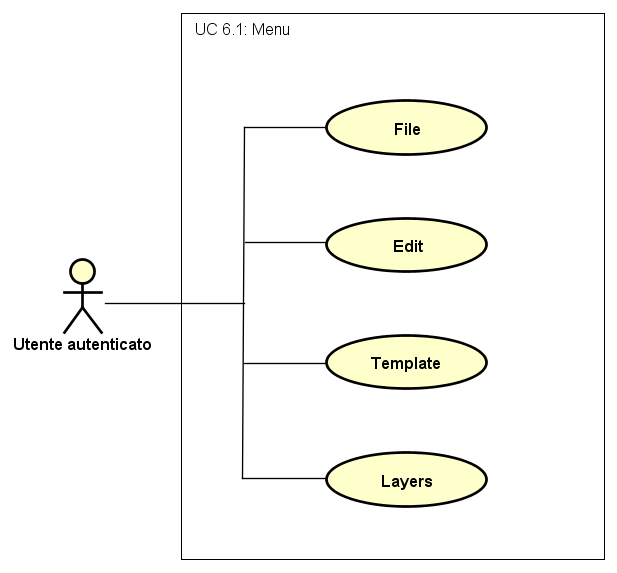
\includegraphics[scale=0.8]{../../Casi D'uso/UC 6.1.png}
\begin{itemize}
		\item \textbf{Attori coinvolti:} Utente autenticato. \\
		\item \textbf{Scopo e descrizione:} L'utente autenticato può accedere alle voci file, edit, tool, layers e window appartenenti al menù del tool designer. \\
		\item \textbf{Precondizione:} L'applicazione offre all'utente una barra dei menù. \\
		\item \textbf{Postcondizione:}L'applicazione, a seconda dell'operazione richiesta dall'utente, svolge le sue funzioni. \\
\end{itemize}